%===================================== CHAP 3 =================================



\chapter{Object Detection}
\label{sec:obj_det}
The problem of detecting objects in an image is harder than classifying an image only containing one object. In object detection, the goal is both to classify objects and locate the exact location of the object in the image. That makes the problem twofold, first we need to find subregions in the image, and then we need to classify them. Since the latter part of the problem has been solved by CNNs, the part that remains is to find these subregions. 

\begin{figure}[h!]
    \centering
    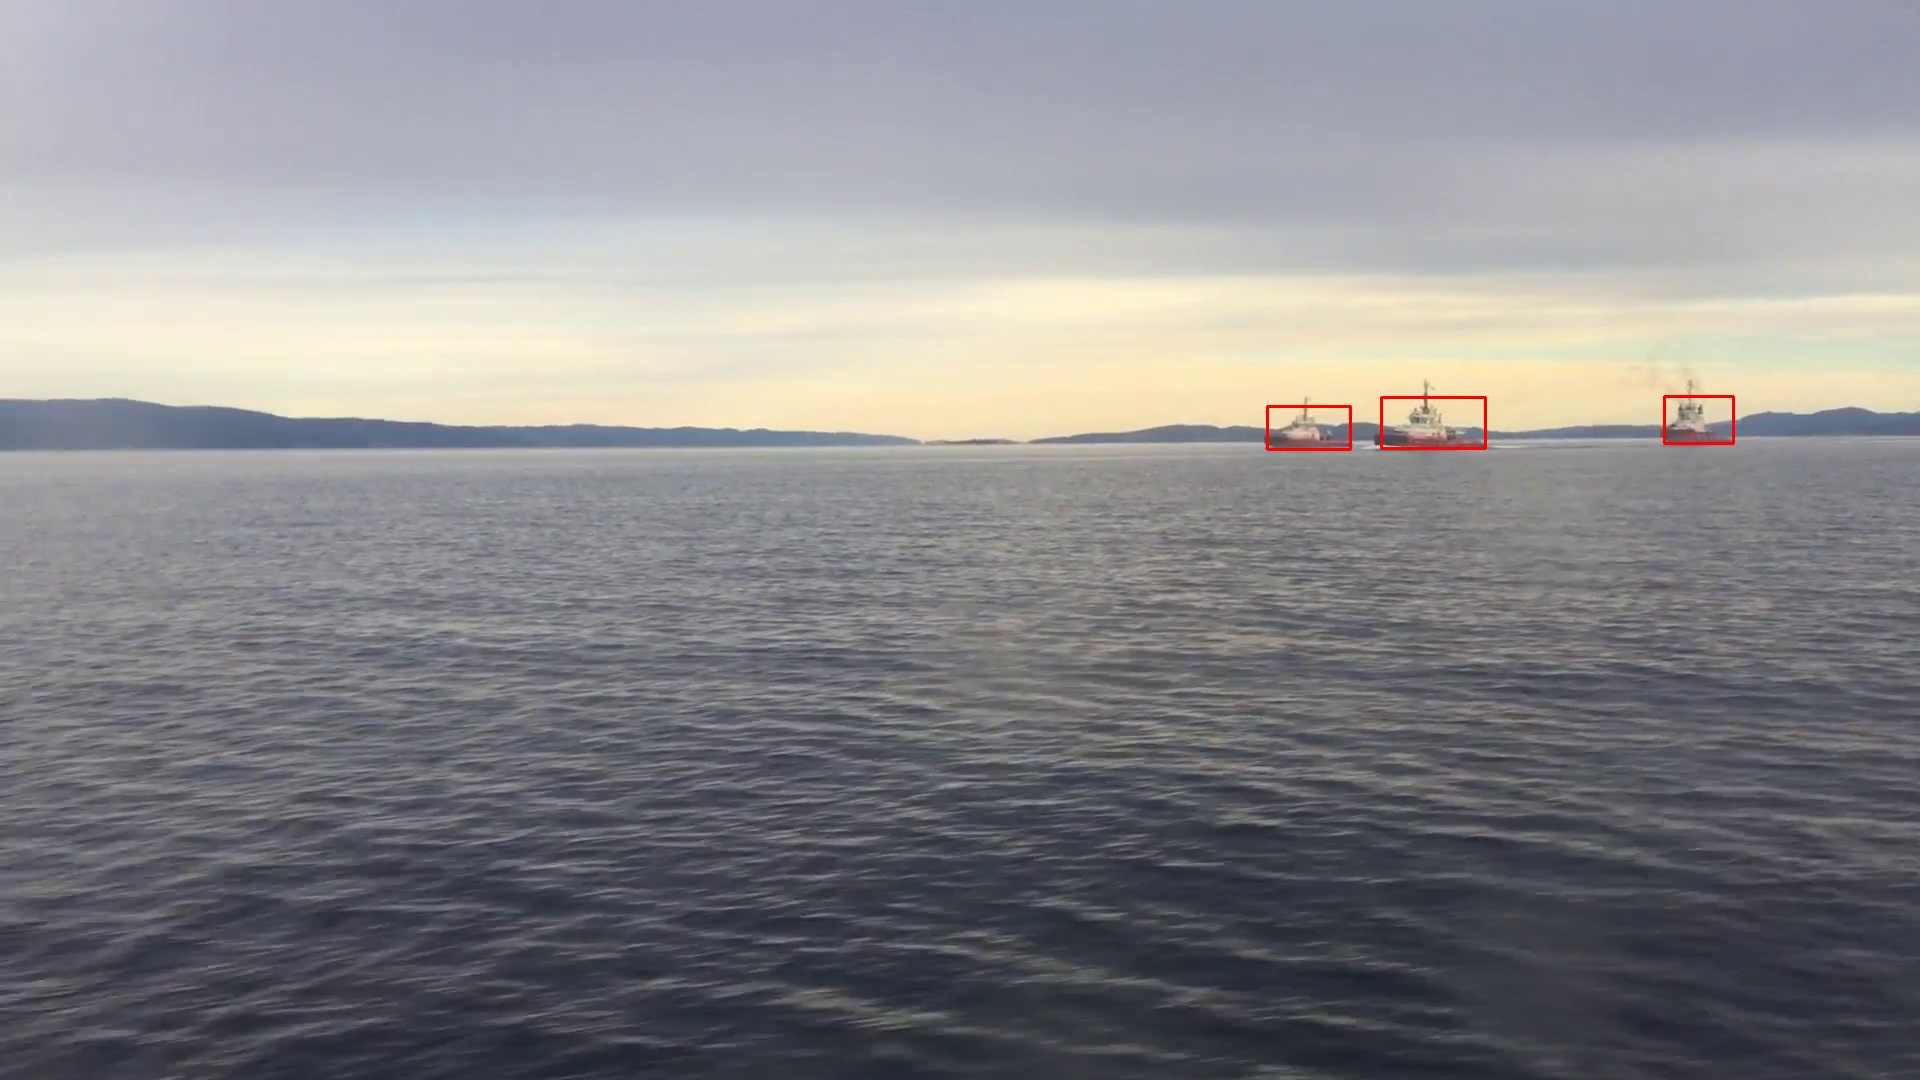
\includegraphics[width = 0.8 \textwidth]{results/video/video3/frame677.jpg}
    \caption{Detected boats.}
    \label{fig:boat_detection}
\end{figure}


\section{Sliding Window (OverFeat)}
The most straightforward solution to find subregions in an image is to use a sliding window, and OverFeat \citep{Sermanet2013} is a method that applies this technique. The sliding window is a window that convolves over the image, like the filters explained in chapter \ref{sec:conv}, and looks at small regions of the image one at a time. This region is then passed through a classification network to determine if this region contains an object of interest. If the classification network returns a high confidence score, OverFeat considers it as an object. 

\vspace{3mm}

The problem with this approach is that it is very computationally exhaustive, and it is also not scale invariant, meaning we have to try several different scales for the sliding windows to be able to detect objects of different sizes. This means that OverFeat has to classify very many subregions, and is therefore not a good option for real-time systems.


\section{R-CNN - Regions with Convolutional Neural Networks }
R-CNN (Regions with Convolutional Neural Networks  \citep{R-CNN}), attacks the problem differently than OverFeat. Instead of trying arbitrary subregions, they propose a solution using the Selective Search algorithm for region proposals.

\subsection{Selective Search }
The Selective Search algorithm \citep{SelSearch} groups adjacent pixels based on color, texture, and intensity together and creates segmented pictures as shown in figure \ref{fig:sel_serach}. It is designed to have a very high recall, meaning that it is acceptable to suggest several false positives, as long as it gets all the true positives. Recall is explained further in chapter \ref{sec:prec_rec}.

\begin{figure}[h!]
    \centering
    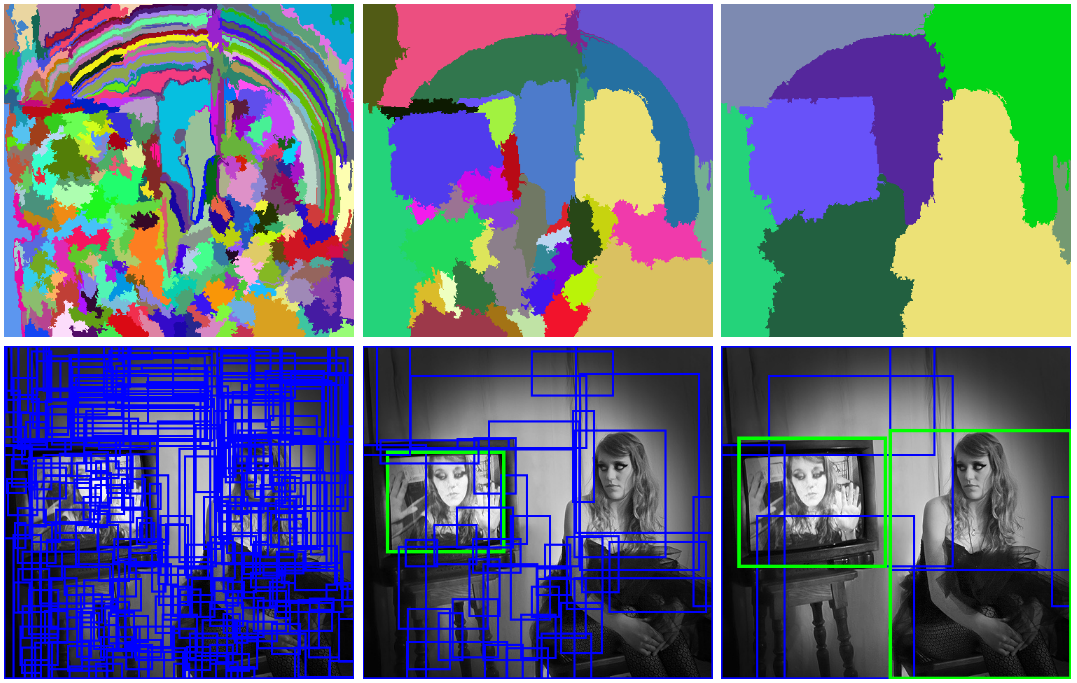
\includegraphics[width=0.8 \textwidth]{fig/sel_search.png}
    \caption{Segmented regions shown in top row, and bounding boxes returned shown in bottom row. This shows why different scales of segmentation is important, since bigger objects are only detected when the image is less segmented. Image from \citep{SelSearch}.}
    \label{fig:sel_serach}
\end{figure}

The Selective Search algorithm takes a segmented image as initial input and performs the following steps:
\begin{enumerate}
  \item Add bounding boxes corresponding to segmented parts to the list of region proposals. This means that regions with the same color (as shown in figure \ref{fig:sel_serach}) will be grouped in a bounding box. A bounding box is a rectangular box that surrounds a potential object.
  \item Group adjacent segments based on similarity.
  \item Go to step 1.
\end{enumerate}


After Selective search has created the region proposals, R-CNN inputs these to a convolutional neural network. The CNN classifies all the region proposals, and if the confidence of the classification is high, the bounding box with its class is outputted from the algorithm. 


\section{Fast R-CNN}

Two years after the release of R-CNN, Fast R-CNN  \citep{FastR-CNN} was released by the same author. In this time he had discovered two drawbacks with R-CNN and found solutions to the problems. 

\begin{enumerate}
    \item R-CNN consists of three different models that all have to be trained. In addition to the CNN, R-CNN consists of a Support Vector Machine (SVM) for classification, and a bounding box regressor, which tightens the bounding boxes around detected objects. Since R-CNN consists of three parts that are trained independently, it makes it harder to train the network as a whole. This is because they are optimizing for themselves and not for the entire system. 
    \subsubsection{Solution to Problem 1}
Instead of training the three parts of the network individually, Fast R-CNN changed the structure in a way that let the whole system be trained together.
     
    \item The CNN has to run once for every region proposal from Selective Search. Since Selective Search is designed to have a very high recall, this ends up being a bottleneck. 
    \subsubsection{Solution to Problem 2}
Instead of calculating the CNN features for every subregion of the image, the CNN features for the entire image were calculated once. Then the features of every region were extracted from this feature map.
\end{enumerate}







\section{Faster R-CNN }
The bottleneck in Fast R-CNN was the region proposals and the Selective Search algorithm. The idea behind Faster R-CNN \citep{FasterR-CNN} is that the region proposals should depend on the features calculated by the CNN. So instead of using Selective Search, we can use the feature maps outputted from the CNN. The feature maps are then inputted in a Region Proposal Network (RPN), which uses a sliding window over the CNN feature map, and outputs \textit{k} potential bounding boxes and scores for how right these boxes are expected to be. These proposals are then fed into the same classifier as used in Fast R-CNN. The difference between the two is just that the region proposals depend only on CNN features in Faster R-CNN. Thus it bypasses the Selective Search algorithm.



\section{YOLO - You Only Look Once }
\label{sec:yolo}
What separates YOLO \citep{YOLOv1}, \citep{YOLOv2} and \citep{YOLOv3} from R-CNN methods is that YOLO only looks once at the picture, and there is only one network for the entire detection process. "We reframe object detection as a single regression problem, straight from image pixels to bounding box coordinates and class probabilities. Using our system, you only look once (YOLO) at an image to predict what objects are present and where they are." \citep{YOLOv1}. 
\vspace{0.5cm}

Yolo starts by dividing the input image into an \textit{S}x\textit{S} grid. The goal for each cell is to predict B bounding boxes and confidence scores for these boxes. If an object has its center in a cell, that cell is responsible for detecting that object. The score of the box says how confident it is that the bounding box contains an object and how accurate it thinks the box is. 

\begin{equation}
    \text{Confidence score} = \text{P(Object)} \cdot \text{IoU}
\end{equation}

IoU is the \textit{Intersect over Union} between the predicted box and ground truth, shown in figure \ref{fig:IoU}. Ground truth is here a manually drawn box over a correct object in the image.


\begin{figure}[h!]
\centering
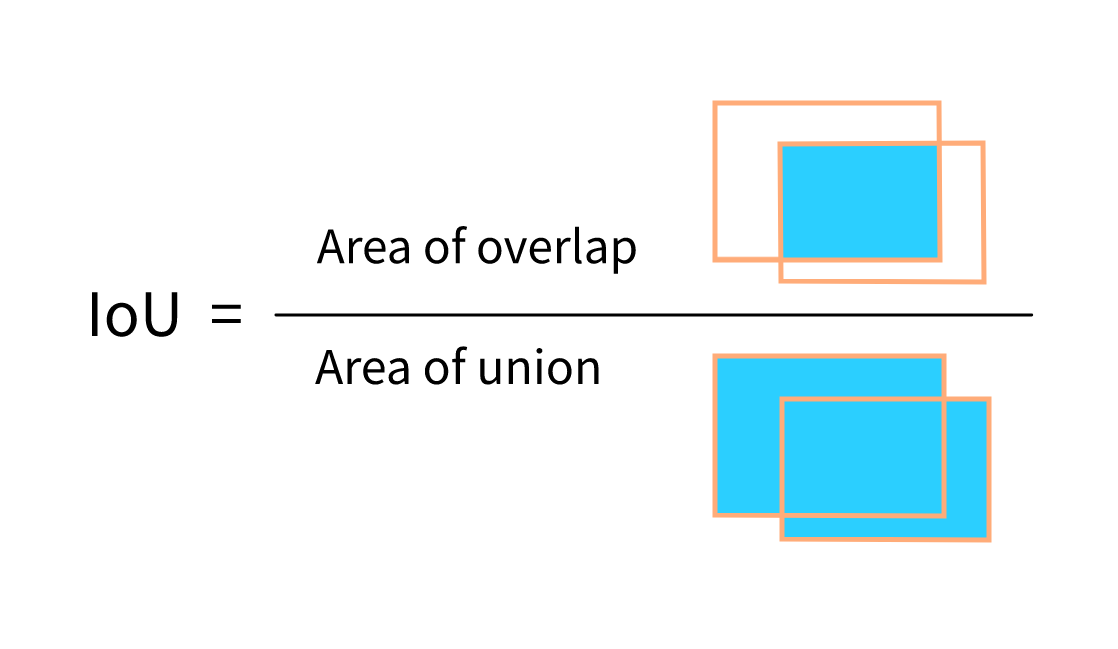
\includegraphics[width=0.8 \textwidth]{fig/iou2.png}
\caption{Intersect over Union}
\label{fig:IoU}
\end{figure}

Each grid cell also predicts C conditional class probabilities, which are conditional on that cell containing an object. 

\begin{equation}
  \text{P(Class}|\text{Object)}
\end{equation}


For each cell, only one set of class probabilities is calculated. To get class specific scores for each bounding box, we multiply these together. 

\begin{equation}
    \text{P(Class}|\text{Object)} \cdot \text{P(Object)} \cdot \text{IoU}
    \label{eq:yolo}
\end{equation}

This gives a value of how well the predicted box fits the object and the probability of that class appearing in the box. When we have this value, we can set a threshold, and only use the results that are probable as output. This is shown in figure \ref{fig:yolo_flow}.  

\begin{figure}[h!]
\centering
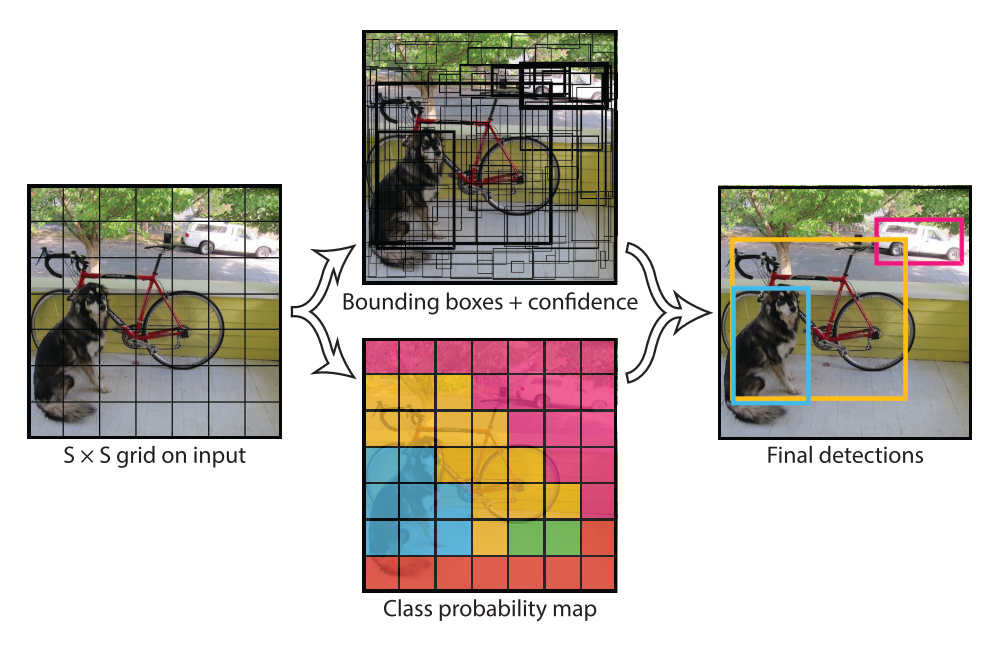
\includegraphics[width=0.8 \textwidth]{images/yolo_flow.png}
\caption{YOLO flow, Top image shows predicted bounding boxes, the thicker the line the higher the confidence score. The bottom picture shows the class probability map. These combined together gives the output image, (Equation \ref{eq:yolo}), image from \citep{YOLOv1}}
\label{fig:yolo_flow}
\end{figure}

%\subsection{Limitations and possible solution}
%The way YOLO grids the input image has several advantages, but also comes with some drawbacks. As mentioned earlier, each cell can only predict one class, and also predicts a limited amount of bounding boxes. Hence, YOLO struggles with small objects that lie close together. I tried running YOLO on some images gotten online, and it seems like this could be a problem for boats that are far away. In figure \ref{fig:pred} one of the boats in the top right corner is not detected. But if I zoom in on that part of the image, and run it through the same network, I get the results shown in figure \ref{fig:pred2}. Here are the bounding boxes more accurate, and it detects a man standing on the foremost boat as well. YOLO does not seem to have a problem with the lowered resolution. 


\newpage

\section{SSD - Single shot Multibox Detector}
The Single Shot Multibox Detector works similarly as YOLO compared to Faster R-CNN. SSD does not use a region proposal network, but as YOLO, it discards the proposal generation step and does all the computation in a single network. A difference between YOLO and SSD is that SSD uses different aspect ratios and scales when it grids the input image, which makes it easier to handle objects of different sizes. By circumventing the proposal generation, SSD saves computational time and runs at a frame rate six to eight times higher than Faster R-CNN with similar accuracy, according to \citep{SSD}. 



Figure \ref{fig:ssd_training} shows how SSD detects objects with different sizes using different aspect ratios on the feature map. Each cell in the feature maps tries different \textit{anchors}, that is proportional to the cell size. The \textit{anchors} are the default boxes shown with dotted lines in figure \ref{fig:ssd_training}. The smallest ground truth object in the image was found in the eight by eight grid, while the bigger object is found using the four by four grid, illustrating how different grid sizes detects objects of different size. The anchors for each cell are run through a classifier which gives a confidence score if multiple boxes predict the same class and have a intersect over union of more than 0.5 the bounding box that has the highest confidence score is chosen. This process is called \textit{non-maximum suppression}.

\begin{figure}[h!]
    \centering
    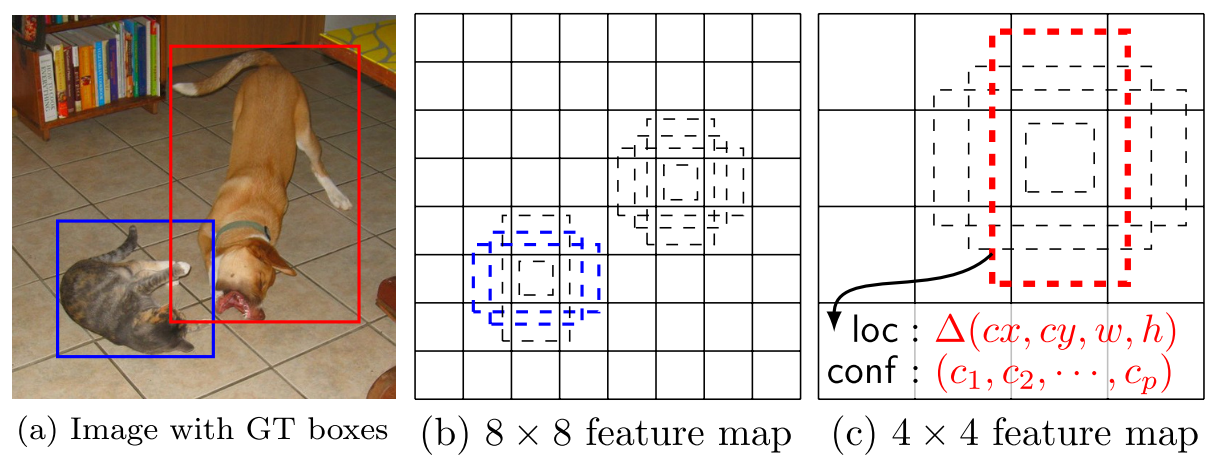
\includegraphics[width=0.9 \textwidth]{images/ssd_train.png}
    \caption{SSD training process, image from \citep{SSD}}
    \label{fig:ssd_training}
\end{figure}

\newpage

\section{Object Detection in Maritime Environments}
\label{sec:obj_det}

Several approaches have been proposed for solving the challenge of object detection in maritime environments. Here, the methods have been divided into deep learning-based methods and algorithms based on traditional computer vision methods (Traditional CV). 

\subsection{Traditional Computer Vision Methods}

\subsubsection{Background Modelling}
Background modeling methods aim to model the background to detect foreground or moving objects. In \citep{BackgroundWaveletSubstract} the authors propose a method for detecting boats using dynamic background modeling and shadow suppression to detect boats. \citep{SeeCoast} and \citep{Pires2010} use background modelling for port surveillance. \citep{Tran2016} uses background subtraction to detect moving boats, and saliency detection to detect non-moving boats. These results are finally fused to generate the detected boats in the scene. All these methods rely on a stationary camera to model the background, and is therefore not likely to perform well on an autonomous ferry.

\subsubsection{Appearance-based Methods}
Appearance-based methods seek to model the vessels appearance and to classify it. These methods extract features from the boats using edge-detection, or other traditional CV-based methods, to detect boats. \citep{HOGdetection} uses HOG-like features and background subtraction together to identify and localize boats. \citep{HAARdetection} detects boats from a rotatable camera using HAAR-like features. \citep{RIBDetection} detects small, fast-moving RIBs by using thermal cameras sensitive different bands of the infrared spectre. While these methods have good results in controlled environments, they are susceptible to noise like sun glare, lighting conditions and other non-optimal weather conditions. 


\subsection{Deep Learning-based Methods}
Earlier in this chapter Faster-RCNN, Yolo and SSD were presented, these are general purpose deep learning-based object detectors. They can be trained on new data, to repurpose them as specialiszed object detectors, such as e.g. a boat detector. There also exist several similar algorithms, and they all can be separated into two categories:

\begin{enumerate}
\item Region proposal based methods, which include R-CNN \citep{R-CNN}, Fast R-CNN \citep{FastR-CNN}, Faster R-CNN \citep{FasterR-CNN}, R-FCN \citep{R-FCN}, Mask R-CNN \citep{MaskRCNN}
\item Regression/classification based methods, which include SSD \citep{SSD}, YOLO \citep{YOLOv1}, \citep{YOLOv2}, \citep{YOLOv3}, MultiBox \citep{Multibox} and RetinaNet \citep{Retinanet}
\end{enumerate}


\citep{SSD_detection2018} aims to develop a real-time detection and tracking system for surveillance cameras in harbours. They have gathered a dataset of 48,966 images containing 70,513 ships from several viewpoints and trained a detector based on SSD to perform detection \citep{SSD}. 

\vspace{3mm}

In \citep{VanEtten2018}, a combination of traditional CV methods and Deep Learning based methods are used to detect boats in satellite images. Large parts of the satellite images do not contain boats, while smaller subframes contains many boats. The solution is to find these subframes by using edge detection methods and then run YOLO. This problem is to some degree relatable to the issue of detecting boats from ships. However, satellite images are less prone to background noise, e.g., from waves. Thus, running the same edge detection algorithms on images taken at sea level returns a lot of noise, and the result is therefore hard to replicate with the same success.

\vspace{3mm}

In \citep{Goring2017}, deep learning-based detection algorithms are trained and tested on detecting maritime navigational markers. In this work they also review of how this can be implemented on a boat, with hardware specifications, is also done. 


\subsection{Challenges in Detection of Maritime Vessels}

In \citep{Challenges2016} a thorough review of the challenges in video based object detection in a maritime scenario is presented. The paper focuses on challenges regarding horizon detection, background subtraction, foreground detection and tracking. While this paper gives a good indication of where traditional CV methods has trouble detecting maritime vessels, it does not address the same problem for deep learning-based methods. It discusses how noise in the background, like wakes, foams, clouds, etc. can make the detection process hard. It also discusses how the maritime scene is affected by illumination conditions such as sunlight, twilight conditions, night, rain, haze, fog, etc. and thus making a model suitable for one weather condition useless for a different environment. Similar research done for deep learning-based methods has not been found.




\subsection{Vehicle Detection for Autonomous Cars}

The field of vehicle detection for autonomous cars is in some ways similar to detection of maritime vessels. While the environment around the object of interest is different and has their own unique challenges, there are similarities in how the desired finished product should be. 

\vspace{3mm}

For vehicle detection a benchmark suite has been developed. \citep{KITTI} provides a platform to "develop novel challenging benchmarks for the tasks of stereo, optical flow, visual odometry / SLAM, and 3D object detection" called KITTI. KITTI simplifies the process of testing new detection algorithms and evaluating performance against previously tested algorithms. It also provides data of which scenarios the detection algorithms perform well, and where it struggles. This gives an indication of how trustworthy the detector will be in a real scenario, also in different environments. On the KITTI website there are links to the highest performing object detectors, with information on how they were implemented.

\vspace{3mm}

In \citep{Wedel2007} video is used to verify obstacles, and to find obstacle boundaries, to supplement radar signals for autonomous cars. \citep{Sun2006} gives a thorough review of the detection methods used for autonomous cars. 


\subsection{Common Challenges in Maritime Object Detection}
Summed up there are many different approaches to the problem of detecting boats in images. A problem with these articles is that even though they give performance metrics on their dataset, there is no way of concluding that their solution will perform as well in other environments. \citep{SSD_detection2018} for instance, trains an SSD detector for detection of boats, it discusses how the detector performs on boats of different sizes, and it also mentions that it performs worse in "difficult situations such as low light, tiny ships and clutter from in-harbor ships". Still, the only performance statistic provided is how well the detector performs on the entire dataset. This indicates that SSD can be a good option. However, an object detector meant to supplement other sensors on an autonomous ship should have known performance statistics in different environments and under different conditions to be reliable in a real scenario. 

\vspace{3mm}

For object detectors to be sufficiently trustworthy and implemented on an autonomous ferry there needs to be well known performance statistics. If the performance statistics in for instance foggy conditions are unknown, the object detector is practically useless under these conditions. Even if the detector performs well, there is no way of telling if the detections are wrong or right whether there is no data supporting the robustness of the output.

\vspace{3mm}

A platform such as KITTI \citep{KITTI} for detection of maritime vessels could be highly useful to get the required performance statistics. Such a system could be used to investigate how different training data affects the performance of the algorithm in different environments, how different detection algorithms compare to each other, and to set clear benchmarks for future re.search



\cleardoublepage